\documentclass[black,white]{beamer}
\usepackage{beamerthemesplit}
\usepackage{amsmath}
\usepackage{adjustbox}
\usepackage{bookmark}
\usepackage{courier}
\usepackage[T1]{fontenc}
\usepackage{hyperref}
\usepackage[utf8]{inputenc}
\usepackage{listings}
\usepackage{lmodern}
\usepackage{tikz}
\usepackage{hyperref}
\usepackage{listings}
\usepackage{lmodern}
\usepackage{pifont}
\usepackage{subcaption}
\usepackage{svg} % Requires inkscape
\usepackage{tikz}
\usetikzlibrary{mindmap}
\usepackage{verbatim}
\usepackage{xcolor}
\usepackage{yaml}

\beamertemplatenavigationsymbolsempty
\usecolortheme{dove}
\useoutertheme{infolines}
\useinnertheme{rectangles}

\newcommand{\cmark}{\ding{51}}%
\newcommand{\bigcmark}{{\large\textcolor{green}\cmark}}
\newcommand{\xmark}{\ding{55}}
\newcommand{\bigxmark}{{\large\textcolor{red}\xmark}}
\newcommand\blfootnote[1]{%
  \begingroup
  \renewcommand\thefootnote{}\footnote{#1}%
  \addtocounter{footnote}{-1}%
  \endgroup
}

%\makeatletter
%\def\blfootnote{\xdef\@thefnmark{}\@footnotetext}
%\makeatother

\definecolor{ashgrey}{rgb}{0.7, 0.75, 0.71}
\definecolor{charcoal}{rgb}{0.21, 0.27, 0.31}
\definecolor{powderblue}{rgb}{0.69, 0.88, 0.9}
\definecolor{layerblue}{RGB}{213, 234, 254}
\newcommand\sectioncolor{\setbeamercolor{background canvas}{bg=layerblue}}

\let\oldhash\#%
\DeclareRobustCommand{\#}{\adjustbox{valign=B,totalheight=.57\baselineskip}{\oldhash}}%

\title[Scaling container policy with eBPF]{Scaling container policy management with kernel features}
\institute{Cilium.io}
\author[Joe Stringer]{Joe Stringer}

\setbeamertemplate{footline}
{
    \leavevmode%
    \hbox{%
        \begin{beamercolorbox}[wd=.333333\paperwidth,ht=2.25ex,dp=1ex,center]{author in head/foot}%
            \usebeamerfont{author in head/foot}\insertshortauthor
        \end{beamercolorbox}%
        \begin{beamercolorbox}[wd=.333333\paperwidth,ht=2.25ex,dp=1ex,center]{title in head/foot}%
            \usebeamerfont{title in head/foot}\insertshorttitle
        \end{beamercolorbox}%
        \begin{beamercolorbox}[wd=.333333\paperwidth,ht=2.25ex,dp=1ex,right]{date in head/foot}%
            \usebeamerfont{date in head/foot}\insertshortdate{}\hspace*{2em}
            \insertframenumber{} / \inserttotalframenumber\hspace*{2ex}
        \end{beamercolorbox}}%
        \vskip0pt%
}

\newcommand\newsectionpage[1]{
    \section{}
    {\sectioncolor
        \begin{frame}
            \vfill
            \centering
            \section{#1}
            \begin{beamercolorbox}[sep=8pt,center,shadow=true,rounded=true]{title}
                \usebeamerfont{title}\insertsectionhead\par%
            \end{beamercolorbox}
            \vfill
        \end{frame}
    }
    \section{#1}
}

\newcommand\suspense{
    \pause $\rightarrow$
}

\date[Sep 11, 2019]{Linux Plumbers 2019, Lisbon, Portugal}

%\begin{filecontents*}{../label-selector.go}
%import{../label-selector.go}
%\end{filecontents*}

\begin{filecontents*}{../sw-l3-l4-policy.yaml}
import{../sw-l3-l4-policy.yaml}
\end{filecontents*}

\begin{document}
    {\sectioncolor
    \begin{frame}
        \titlepage
        \begin{figure}
            
\includegraphics[scale=0.2]{lpc-logo.png}
        \end{figure}
    \end{frame}
    }

    %\logo{\includesvg[scale=0.4]{cilium-logo.svg}}

    \begin{frame}{Agenda}
        \begin{itemize}
            \item Architecture \medskip
            \item Policy model \medskip
            \item Datapath model \medskip
        \end{itemize}
    \end{frame}

    \begin{frame}{Kubernetes Architecture 101}
        \centering
        \vfill
        \begin{figure}
            \includesvg[width=0.8\textwidth,keepaspectratio]{k8s-architecture.svg}
        \end{figure}
        \blfootnote{{\tiny Thomas Graf, {\em Scaling to 5k Kubernetes Nodes: Lessons Learned}, Cloud Native Rejekts EU 2019}}
    \end{frame}

    \begin{frame}{Kubernetes networking plugins}
        \vfill
        \begin{table}
            \begin{subtable}[l]{0.6\textwidth}
                \begin{itemize}
                    \item Plumb local connectivity (CNI) \medskip
                    \item Connect remote nodes \medskip
                    \item Services / loadbalancing \medskip
                    \item Network policy \medskip
                \end{itemize}
            \end{subtable}
            \begin{subtable}[r]{0.35\textwidth}
                \begin{figure}
                    \includesvg[width=0.4\textwidth,keepaspectratio]{cni-logo.svg}
                \end{figure}
            \end{subtable}
        \end{table}
        \vfill
        \blfootnote{{\tiny \url{https://kubernetes.io/docs/concepts/extend-kubernetes/compute-storage-net/network-plugins/}}}
    \end{frame}

    \begin{frame}{Cilium}
        \vfill
        \begin{table}
            \begin{subtable}[l]{0.45\textwidth}
                \begin{itemize} \item Native BPF dataplane \medskip
                    \item Modular architecture \medskip
                    \item API-Aware security model \medskip
                    \item Scalable \medskip
                \end{itemize}
            \end{subtable}
            \begin{subtable}[r]{0.5\textwidth}
                \begin{figure}
                    \includesvg[width=1.1\textwidth,keepaspectratio]{cilium-plugins.svg}
                \end{figure}
            \end{subtable}
        \end{table}
        \vfill
        \blfootnote{{\tiny \url{https://cilium.io/}}}
    \end{frame}

    \begin{frame}{Cluster events}
        \begin{itemize}
            \item Nodes $\rightarrow$ Fabric connectivity \medskip \pause
            \item Pods $\rightarrow$ End-to-end connectivity \medskip \pause
            \item Services $\rightarrow$ Logical connectivity \medskip \pause
            \item Network policies $\rightarrow$ Connectivity isolation \medskip
        \end{itemize}
    \end{frame}

    \begin{frame}{Cluster events}
        \begin{itemize}
            \item Nodes $\rightarrow$ Fabric connectivity \medskip
		    \item \textbf{Pods} $\rightarrow$ End-to-end connectivity \medskip
            \item Services $\rightarrow$ Logical connectivity \medskip
            \item \textbf{Network policies} $\rightarrow$ Connectivity isolation \medskip
        \end{itemize}
    \end{frame}

    \begin{frame}{Pods}
        \begin{itemize}
            \item BPF Templating \medskip
        \end{itemize}
    \end{frame}

    \begin{frame}{ELF Templating}
        \centering
        \includesvg[scale=0.9]{bpf-templating.svg}
    \end{frame}

    \begin{frame}{Policy}
    \end{frame}

    %    \begin{itemize}
    %        \item Nodes \suspense Fabric connectivity \smallskip
    %            \pause
    %            \begin{itemize}
    %                \item Tunnel / Encryption / Direct routing \medskip
    %            \end{itemize}
    %            \pause
    %        \item Pods \suspense End-to-end connectivity \smallskip
    %            \pause
    %            \begin{itemize}
    %                \item Configure local kernel for new network namespace \medskip
    %                \item Allocate identity for pod labels \medskip
    %            \end{itemize}
    %            \pause
    %        \item Services \suspense Logical connectivity \smallskip
    %            \pause
    %            \begin{itemize}
    %                \item Configure service translation \medskip
    %            \end{itemize}
    %            \pause
    %        \item Network policies \suspense Connectivity isolation \medskip
    %    \end{itemize}
    %\end{frame}

    %\begin{frame}{Policy model}
    %    \begin{itemize}
    %        \item Whitelist \medskip
    %        \item L3 \smallskip
    %            \begin{itemize}
    %                \item Pod labels \medskip
    %                \item FQDN \medskip
    %                \item Services \medskip
    %            \end{itemize}
    %        \item L4 \medskip
    %        \item L7 \smallskip
    %            \begin{itemize}
    %                \item HTTP \medskip
    %                \item DNS \medskip
    %                \item Your protocol here \medskip
    %            \end{itemize}
    %    \end{itemize}
    %\end{frame}

    \begin{frame}{Cilium Architecture}
        \centering
        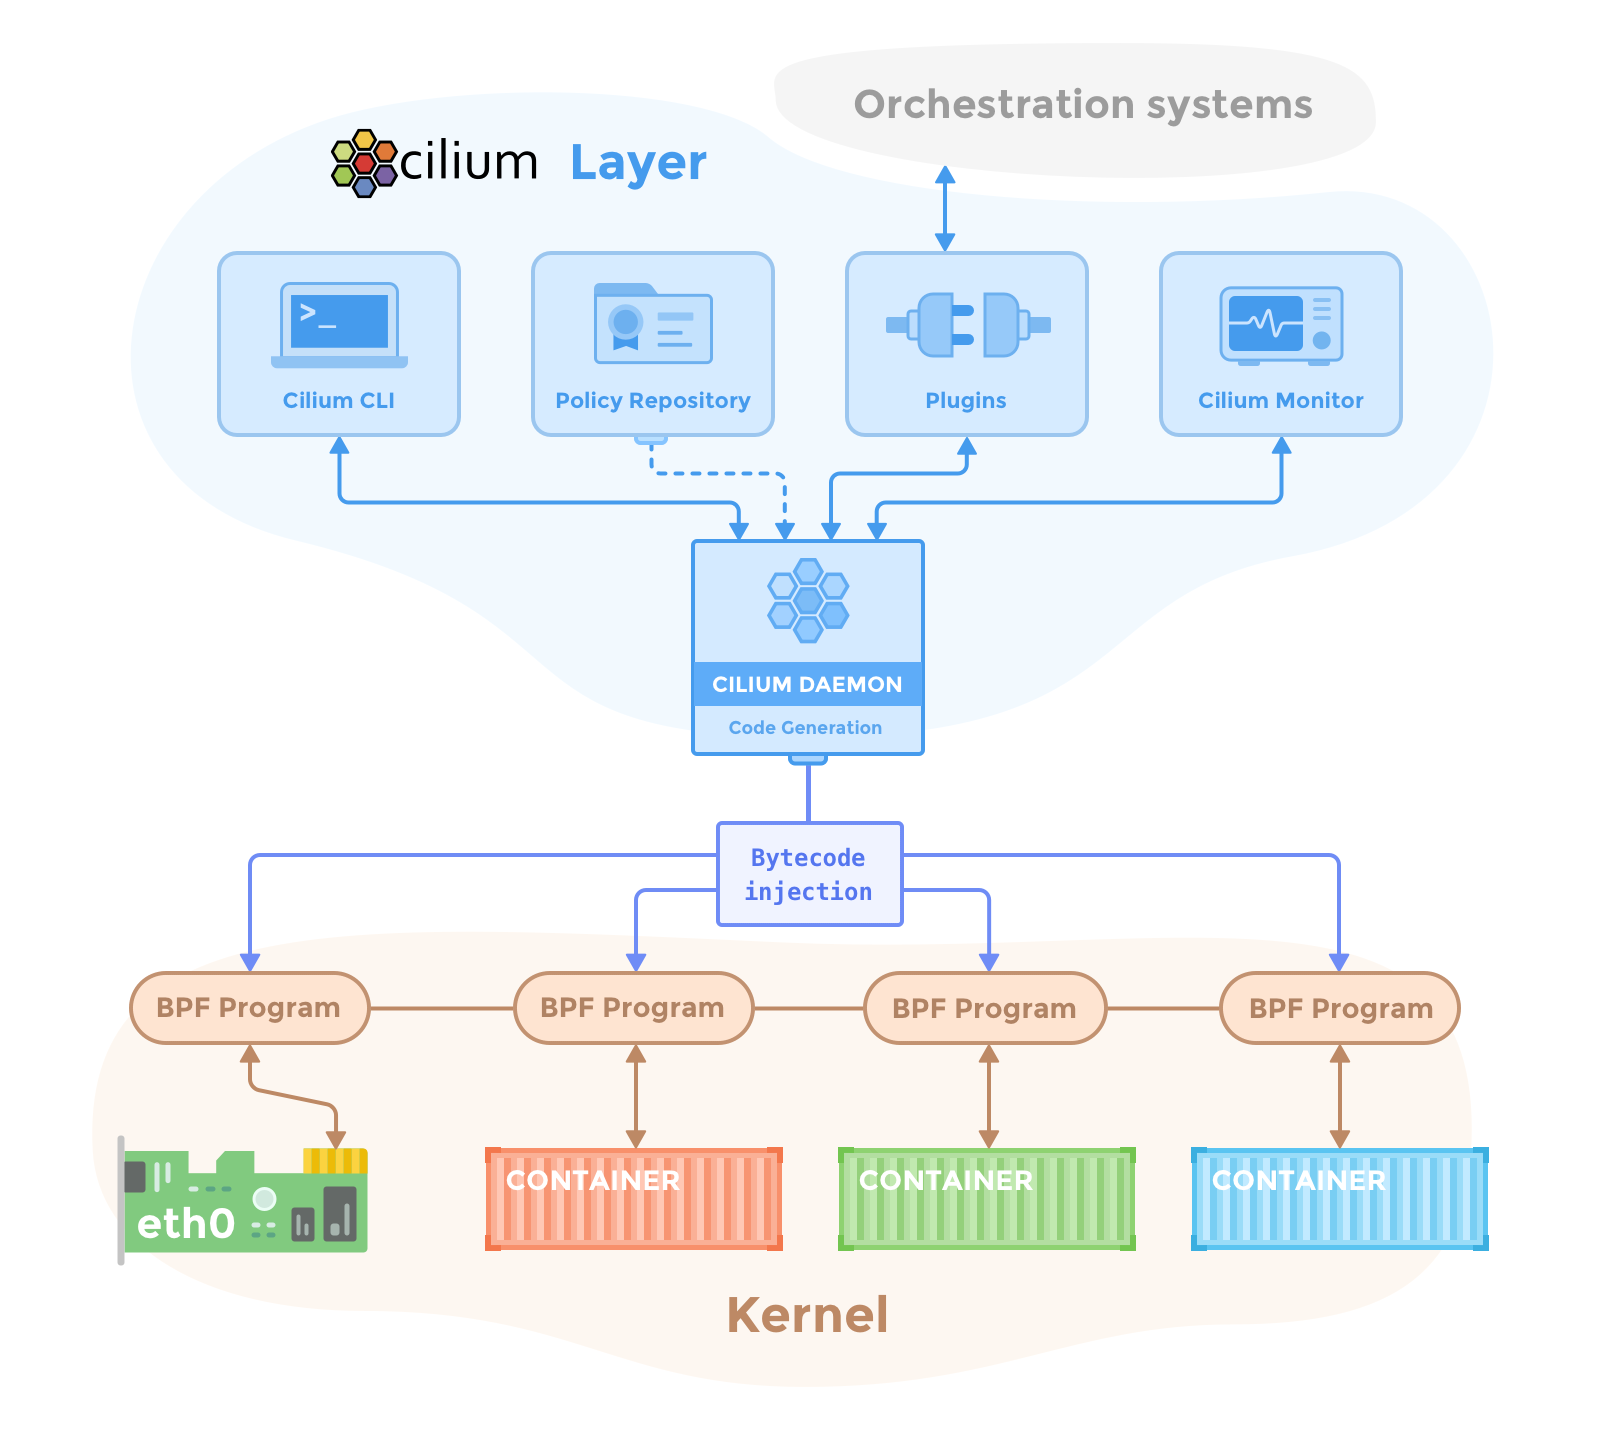
\includegraphics[width=0.8\textwidth,keepaspectratio]{cilium_architecture.png}
    \end{frame}

    \begin{frame}{Identity-based security}
        \centering
        \vfill
        \begin{figure}
            \includesvg[scale=0.7]{identity-security.svg}
        \end{figure}
        \vfill
        \blfootnote{{\tiny Thomas Graf, {\em Cilium \& BPF - The Future of Networking and Security}, openSUSE Conference 2019}}
    \end{frame}

    \begin{frame}{Policy example}
        \lstinputlisting[language=yaml,%
                         showstringspaces=false,%
                         basicstyle=\footnotesize,%
                         breaklines=true]{../sw-l3-l4-policy.yaml}
        \blfootnote{\tiny \url{https://docs.cilium.io/en/stable/gettingstarted/http/}}
    \end{frame}

    %\begin{frame}{Label selection}
    %    \lstinputlisting[language=go,%
    %                     basicstyle=\footnotesize,%
    %                     breaklines=true]{../label-selector.go}
    %    \blfootnote{\tiny \url{https://github.com/kubernetes/apimachinery/blob/master/pkg/apis/meta/v1/types.go}}
    %\end{frame}

    \begin{frame}{... memoization something something ...}
    \end{frame}

    \begin{frame}{Datapath Configuration}
        \centering
        \vfill
        \begin{figure}
        \begin{overprint}
            \onslide<1>\includesvg[scale=0.9]{cilium-bpf-egress-l3.svg}
            \onslide<2>\includesvg[scale=0.9]{cilium-bpf-egress-l7.svg}
            \onslide<3>\includesvg[scale=0.9]{cilium-bpf-egress-proxy.svg}
        \end{overprint}
        \end{figure}
        \vfill
    \end{frame}

    \begin{frame}{L7 Configuration: Attempt \#1}
        \centering
        %\begin{figure}
        %    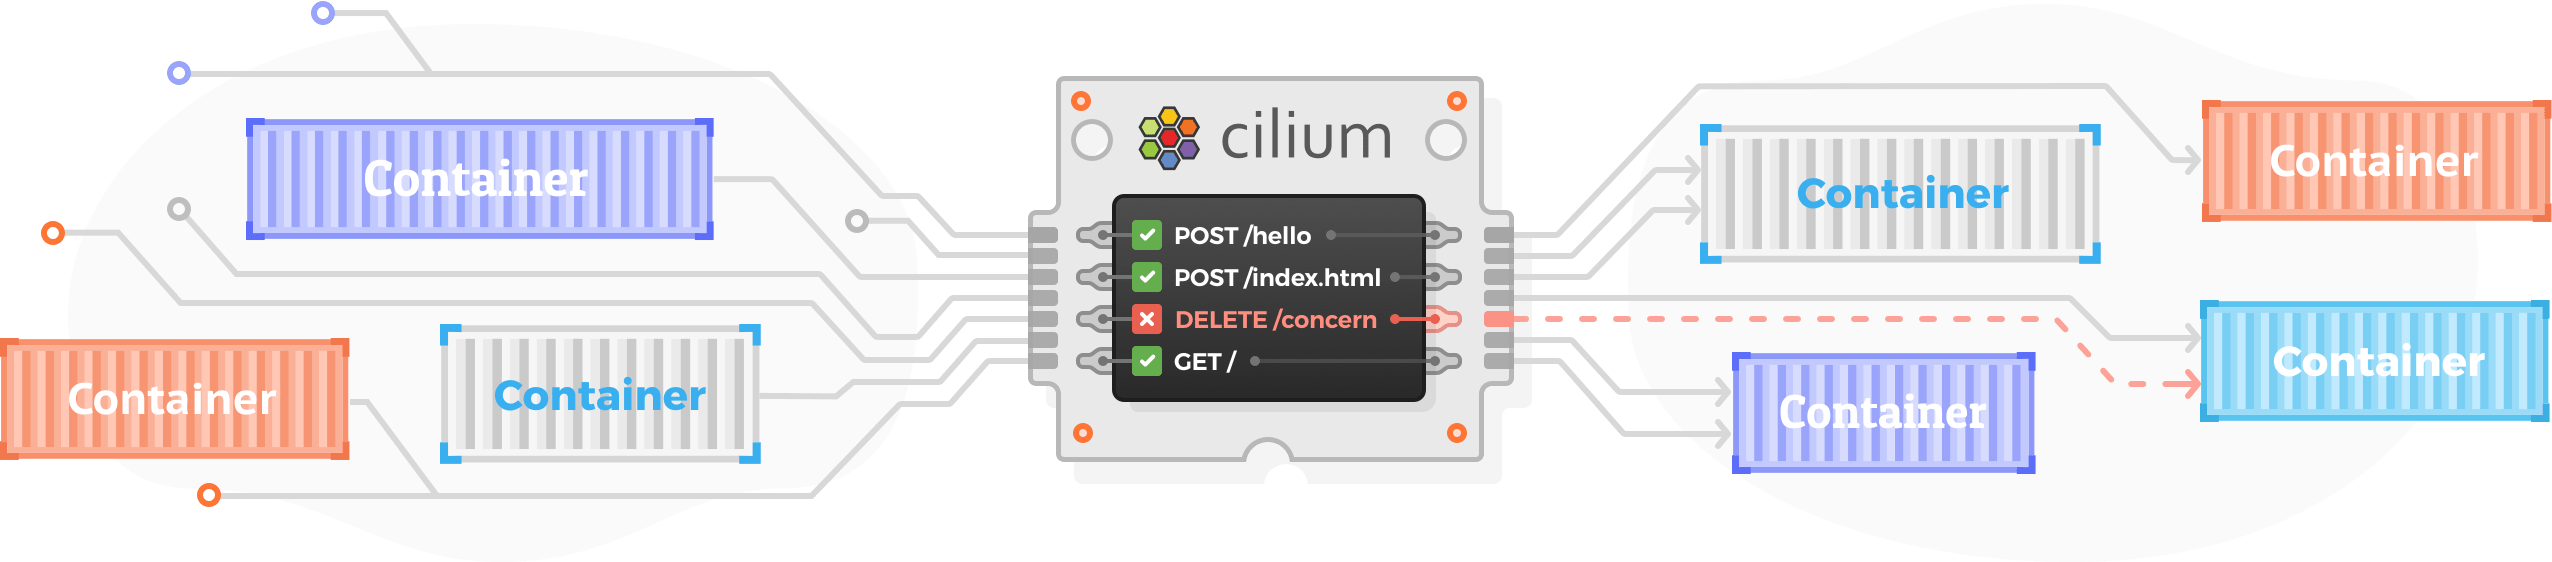
\includegraphics[scale=0.08]{cilium_api_security.png}
        %\end{figure}
        \begin{figure}
        \begin{overprint}
            \centering
            \onslide<1>\includesvg[scale=0.8]{bpf-proxy-nat-0.svg}
            \onslide<2>\includesvg[scale=0.8]{bpf-proxy-nat-1.svg}
            \onslide<3>\includesvg[scale=0.8]{bpf-proxy-nat-2.svg}
            \onslide<4>\includesvg[scale=0.8]{bpf-proxy-nat-3.svg}
        \end{overprint}
        \end{figure}
        \vfill
    \end{frame}

    \section{}
    \begin{frame}{Thank you}
        \vfill
    \centering
    Joe Stringer \\\medskip
    joe@cilium.io
    \vfill
    \end{frame}

\end{document}
